\documentclass[a4paper,12pt]{article}

% Добавляем новые пакеты
\usepackage{pifont}
\usepackage{emoji}

\usepackage[english, russian]{babel}    % Пакет для поддержки русского языка
\usepackage[T1, T2A]{fontenc}           % Загружаем пакет с поддержкой кирилицы
\usepackage[utf8]{inputenc}             % Загружаем пакет с поддержкой кодировки файла и символов
\usepackage{graphicx}                   % Загружаем пакет для добавления различной графики (pdf, jpg, png)
\usepackage{import}                     % Загружаем пакет для продвинутого импорта, в частности изображений pdf_tex из графического редактора inkscape
\usepackage{subcaption}                 % Пакет для поддержки сетки из фигур, например в две колонки или матрицей
\usepackage{float}        
\usepackage{fontawesome}
% Пакет для улучшенного размещения изображенией
\usepackage{geometry}                   % Пакет для управления отступами на странице
\usepackage{amsmath}                    % Добавляем крутую поддержку математики
\usepackage{amsfonts}                   % Пакет с математическими шрифтами
\usepackage{tabu}                       % Пакет с прокаченными таблицами
\usepackage{booktabs}                   % Крутые вертикальные разделители
\usepackage[dvipsnames]{xcolor}         % Расширенная поддержка цветов
\usepackage[colorlinks]{hyperref}
\usepackage{indentfirst}                % Пакет, чтобы починить красную строку
\usepackage{listings}                   % Поддержка листингов, оформления кода программы
    \usepackage{longtable}
\usepackage{makecell}
\usepackage{multirow}
\usepackage{tabularray}
\usepackage{ amssymb }
\usepackage{varwidth}
\usepackage{bm}

\graphicspath{ {./images/} }

% Устанавливает отступы на странице
\geometry{left=2cm, right=2cm, bottom=2cm, top=2cm}

% Настраиваем красивые цвета для ссылок на формулы, фигуры (изображения) и другие элементы.
\hypersetup{
    linkcolor=blue,
    filecolor=magenta,
    urlcolor=cyan
}

% Настраиваем супер красивые листинги
\definecolor{codegreen}{rgb}{0,0.6,0}
\definecolor{codegray}{rgb}{0.5,0.5,0.5}
\definecolor{codepurple}{rgb}{0.58,0,0.82}
\definecolor{backcolour}{rgb}{0.95,0.95,0.92}

\lstdefinestyle{codestyle}{
    backgroundcolor=\color{backcolour},
    commentstyle=\color{codegreen},
    keywordstyle=\color{magenta},
    numberstyle=\tiny\color{codegray},
    stringstyle=\color{codepurple},
    basicstyle=\ttfamily\footnotesize,
    breakatwhitespace=false,
    breaklines=true,
    captionpos=b,
    keepspaces=true,
    numbers=left,
    numbersep=5pt,
    showspaces=false,
    showstringspaces=false,
    showtabs=false,
    tabsize=2
}

\lstset{style=codestyle}
\lstset{extendedchars=\true}

\begin{document}
\begin{titlepage}
    \centering
    \vspace*{1cm}

    {\large Министерство науки и высшего образования Российской Федерации}\\
    {\large ФЕДЕРАЛЬНОЕ ГОСУДАРСТВЕННОЕ АВТОНОМНОЕ ОБРАЗОВАТЕЛЬНОЕ УЧРЕЖДЕНИЕ ВЫСШЕГО ОБРАЗОВАНИЯ «НАЦИОНАЛЬНЫЙ ИССЛЕДОВАТЕЛЬСКИЙ УНИВЕРСИТЕТ ИТМО»}\\
    {\large (УНИВЕРСИТЕТ ИТМО)}\\

    \vspace{2cm}

    {\large Факультет «Систем управления и робототехники»}\\

    \vspace{3cm}

    \textbf{{\Huge ОТЧЕТ}\\
    {\Huge О ЛАБОРАТОРНОЙ РАБОТЕ №1}}\\

    \vspace{1cm}

    {\LARGE По дисциплине «Частотные методы»}\\
    {\LARGE на тему: «Ряды Фурье»}\\

    \vspace{3cm}

    {\Large Студент:}\\
    Охрименко Ева

    \vspace{2cm}

    {\Large Преподаватели:}\\
    Догадин Егор Витальевич\\
    Пашенко Артем Витальевич\\

    \vspace{2cm}

    {\large г. Санкт-Петербург}\\
    {\large 2024}

\end{titlepage}
\newpage
\tableofcontents
\newpage

\definecolor{codeblue}{rgb}{0,0,0.6}
\definecolor{codered}{rgb}{0.6,0,0}
\definecolor{codegreen}{rgb}{0,0.5,0}
\definecolor{codegray}{rgb}{0.5,0.5,0.5}
\definecolor{codebg}{rgb}{0.95,0.95,0.92}

\lstdefinestyle{mystyle}{
    backgroundcolor=\color{codebg},   
    commentstyle=\color{codegreen},
    keywordstyle=\color{codeblue},
    numberstyle=\tiny\color{codegray},
    stringstyle=\color{codered},
    basicstyle=\ttfamily\footnotesize,
    breakatwhitespace=false,         
    breaklines=true,                 
    captionpos=b,                    
    keepspaces=true,                 
    numbers=left,                    
    numbersep=5pt,                  
    showspaces=false,                
    showstringspaces=false,
    showtabs=false,                  
    tabsize=2
}

\lstset{style=mystyle}



\section{Task. Вещественные функции}


Ряд Фурье представляет собой разложение периодической функции \( f(t) \) в сумму синусоидальных и косинусоидальных функций. Для функции с периодом \( T \) разложение имеет вид:

\begin{equation}
f(t) = a_0 + \sum_{n=1}^{\infty} \left( a_n \cos \frac{2\pi n}{T} t + b_n \sin \frac{2\pi n}{T} t \right).
\end{equation}


Коэффициенты \( a_0 \), \( a_n \) и \( b_n \) определяются с помощью интегралов:

\begin{equation}
a_0 = \frac{1}{T} \int_{0}^{T} f(t) \, dt.
\end{equation}

\begin{equation}
a_n = \frac{2}{T} \int_{0}^{T} f(t) \cos \frac{2\pi n}{T} t \, dt.
\end{equation}

\begin{equation}
b_n = \frac{2}{T} \int_{0}^{T} f(t) \sin \frac{2\pi n}{T} t \, dt.
\end{equation}

Функции \( \cos \frac{2\pi n}{T} t \) и \( \sin \frac{2\pi n}{T} t \) образуют ортонормированный базис в пространстве квадратно-интегрируемых функций. Это означает, что любую периодическую функцию можно представить в виде бесконечной суммы таких функций.

\subsection{Квадратная волна}

Сначала сделаю предподготовку к заданию, выберу числа \( a, b, t_0, t_1, t_2 \) такие, что \( a, b > 0 \) и \( t_2 > t_1 > t_0 > 0 \). Мой следующий код будет написан на языке программирования Wolfram Matematica Language.


% Вставка листинга кода Mathematica
\begin{lstlisting}[language=Mathematica, caption={Выбор чисел}]
a = 2;
b = 1;
t0 = 0;
t1 = Pi/2;
t2 = Pi;
T = t2 - t0;
h = 3;
\end{lstlisting}

Далее по заданию мне нужно задать функцию квадратной волны

\begin{lstlisting}[language=Mathematica, caption={Задание функции}]
f[t_] := Piecewise[{{a, 0 <= Mod[t, T] <= t1}, {b, t1 < Mod[t, T] <= t2}}];
\end{lstlisting}

\[
f(t_n) =
\begin{cases} 
2, & 0 \leq \operatorname{Mod}(t_n, \pi) \leq \frac{\pi}{2} \\
1, & \frac{\pi}{2} < \operatorname{Mod}(t_n, \pi) \leq \pi
\end{cases}
\]

где:

\begin{itemize}
    \item \( \operatorname{Mod}(t_n, \pi) \) — остаток от деления \( t_n \) на \( \pi \), создающий периодичность функции.
    \item Если \( \operatorname{Mod}(t_n, \pi) \) находится в интервале \( [0, \frac{\pi}{2}] \), функция принимает значение \( 2 \).
    \item Если \( \operatorname{Mod}(t_n, \pi) \) находится в интервале \( (\frac{\pi}{2}, \pi] \), функция принимает значение \( 1 \).
\end{itemize}

Такой график у меня получился 
\begin{figure}[H]
    \centering
    
\includegraphics[width=0.7\textwidth]{pic/1.png}
    \caption{График частотной волны}
    \label{fig:example_image}
\end{figure}



\subsubsection{Счет первых 2 коэффициентов вручную}
Теперь посчитаю первые 2 коэффициента Фурье вручную

\[
a_0 = \frac{2}{T} \int_{0}^{T} f(t) \, dt = \frac{2}{\pi} \left( \int_{0}^{\frac{\pi}{2}} 2 \, dt + \int_{\frac{\pi}{2}}^{\pi} 1 \, dt \right) = \frac{2}{\pi} \left( \pi + \frac{\pi}{2} \right) = 3
\]

\[
a_1 = \frac{2}{T} \int_{0}^{T} f(t) \cos\left(\frac{2\pi n t}{T}\right) \, dt = \frac{2}{\pi} \left( \int_{0}^{\frac{\pi}{2}} 2 \cos(2t) \, dt + \int_{\frac{\pi}{2}}^{\pi} 1 \cos(2t) \, dt \right) = \frac{2}{\pi} (0 + 0) = 0
\]


\[
b_1 = \frac{2}{T} \int_{0}^{T} f(t) \sin\left(\frac{2\pi n t}{T}\right) \, dt = \frac{2}{\pi} \left( \int_{0}^{\frac{\pi}{2}} 2 \sin(2t) \, dt + \int_{\frac{\pi}{2}}^{\pi} 1 \sin(2t) \, dt \right) = \frac{2}{\pi} (2 - 1) = \frac{2}{\pi} \approx 0.63662
\]

Итоговый ряд Фурье для n = 2:
\[
f(t) \approx \frac{a_0}{2} + b_1 \sin(2t) = 1.5 + 0.63662 \sin(2t)
\]



Коэффициенты \( c_n \) определяются как:

\[
c_n = \frac{1}{T} \int_{0}^{T} f(t) e^{-i \frac{2\pi n}{T} t} dt
\]

Подставляя \( T = \pi \), получаем:

\[
c_n = \frac{1}{\pi} \int_{0}^{\pi} f(t) e^{-i 2 n t} dt = \frac{1}{\pi} \left( \int_{0}^{\frac{\pi}{2}} 2 e^{-i 2 n t} dt + \int_{\frac{\pi}{2}}^{\pi} 1 e^{-i 2 n t} dt \right)
\]

При \( n = 0 \):

\[
c_0 = \frac{1}{\pi} \left( \int_{0}^{\frac{\pi}{2}} 2 dt + \int_{\frac{\pi}{2}}^{\pi} 1 dt \right) = \frac{1}{\pi} \left( 2 \times \frac{\pi}{2} + (\pi - \frac{\pi}{2}) \right) = \frac{3}{2}
\]

Для \( n = 1 \):

\[
c_1 = \frac{1}{\pi} \left( \int_{0}^{\frac{\pi}{2}} 2 e^{-i 2 t} dt + \int_{\frac{\pi}{2}}^{\pi} 1 e^{-i 2 t} dt \right)
\]

\[
= \frac{1}{\pi} \left( 2 \times \frac{e^{-i \pi} - 1}{-2i} + \frac{e^{-i 2\pi} - e^{-i \pi}}{-2i} \right) = \frac{1}{\pi} \left( -i - i \right) = -\frac{2i}{\pi}
\]

Для \( n = 2 \):

\[
c_2 = \frac{1}{\pi} \left( \int_{0}^{\frac{\pi}{2}} 2 e^{-i 4 t} dt + \int_{\frac{\pi}{2}}^{\pi} 1 e^{-i 4 t} dt \right)
\]

\[
= \frac{1}{\pi} \left( \frac{2}{-4i} (e^{-i 2\pi} - 1) + \frac{1}{-4i} (e^{-i 4\pi} - e^{-i 2\pi}) \right) = \frac{1}{\pi} (0) = 0
\]

Итоговое разложение:

\[
f(t) \approx \frac{c_0}{2} + c_1 e^{i 2t} + c_{-1} e^{-i 2t}
\]

Так как \( c_{-1} = \overline{c_1} = \frac{2i}{\pi} \), получаем:

\[
c_1 e^{i 2t} + c_{-1} e^{-i 2t} = -\frac{2i}{\pi} e^{i 2t} + \frac{2i}{\pi} e^{-i 2t} = -\frac{2i}{\pi} (\cos 2t + i \sin 2t) + \frac{2i}{\pi} (\cos 2t - i \sin 2t)
\]

\[
= -\frac{2i}{\pi} \cos 2t - \frac{2}{\pi} \sin 2t + \frac{2i}{\pi} \cos 2t - \frac{2}{\pi} \sin 2t = -\frac{2}{\pi} \sin 2t
\]

Итоговый ряд:

\[
f(t) \approx \frac{3}{2} - \frac{2}{\pi} \sin 2t
\]


Можно заметить, что, разложение через вещественные и комплексные коэффициенты эквивалентно, что подтверждает равенство их значений.



\subsubsection{Автоматизация}

Теперь приступлю к написанию кода и отрисовки графиков для различных коэффициентов n (n берется за частоту гармоник).




\begin{lstlisting}[language=Mathematica, caption={Код для квадратной волны}]
n = 5;

A0 = (2/T) Integrate[f[t], {t, 0, T}];

A[k_] := (2/T) Integrate[f[t] Cos[(2 Pi k t)/T], {t, 0, T}];
B[k_] := (2/T) Integrate[f[t] Sin[(2 Pi k t)/T], {t, 0, T}];

A0val = N[A0];
Avals = Table[N[A[k]], {k, 1, n}];
Bvals = Table[N[B[k]], {k, 1, n}];

fourierSeries = 
  A0val/2 + 
   Sum[Avals[[k]] Cos[(2 Pi k t)/T] + 
     Bvals[[k]] Sin[(2 Pi k t)/T], {k, 1, n}];

c[n_] := (1/T) Integrate[f[t] Exp[-I (2 Pi n t)/T], {t, 0, T}];

cVals = Table[N[c[k]], {k, -n, n}];

fourierSeriesComplex = 
  A0val/2 + 
   2 Sum[Re[cVals[[k + n + 1]]] Cos[(2 Pi k t)/T] - 
      Im[cVals[[k + n + 1]]] Sin[(2 Pi k t)/T], {k, 1, n}];

Plot[{fourierSeries, fourierSeriesComplex, f[t]}, {t, 0, 3*T}, 
 PlotStyle -> {{Thick, Blue}, {Thick, Dashed, Red}, {Thick, Green}}, 
 PlotLegends -> {"Тригонометрическое разложение (A + B)", 
   "Комплексное разложение (c_n)", "Оригинальная функция"}, 
 AxesLabel -> {"t", "y"}, PlotRange -> All, Exclusions -> None]

\end{lstlisting}

После выполнения кода у меня нарисуется график квадратной волны и на нем же отрисуются оба разложения Фурье. \\
Ряды запишутся в переменные \( fourierSeries\) и \( fourierSeriesComplex \) .

\begin{figure}[H]
    \centering
    
\includegraphics[width=0.4\textwidth]{pic/2.png}
    \caption{Вывод программы. Ряды}
    \label{fig:example_image}
\end{figure}

Как можно заметить, ряды получились одинаковые, следовательно, все сделано верно.
Теперь оценим получившийся график


\begin{figure}[H]
    \centering
    
\includegraphics[width=0.9\textwidth]{pic/3.png}
    \caption{График квадратной волны и апроксимированные}
    \label{fig:example_image}
\end{figure}

Все сходится, значит задание успешно выполнено. Единственное, при n = 2, аппроксимация не такая сильная. Давайте рассмотрим графики для n побольше.

\subsubsection{Графики квадратной волны для больших n}


\begin{figure}[H]
    \centering

    \subfloat[n = 4]{%
        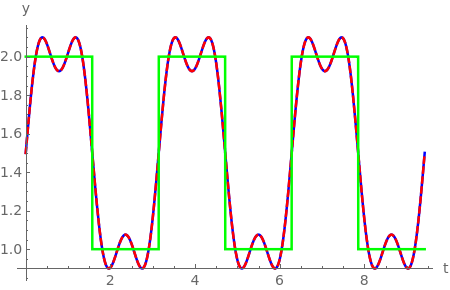
\includegraphics[width=0.45\textwidth]{pic/n4.png}
    }
    \hfill
    \subfloat[n = 5]{%
        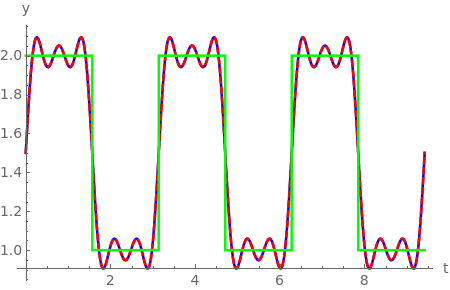
\includegraphics[width=0.45\textwidth]{pic/n5.png}
    }
    
    
    \vskip 0.5cm  
    \subfloat[n = 7]{%
        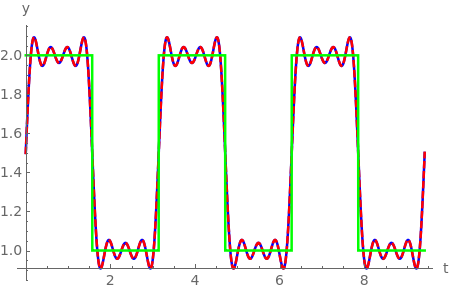
\includegraphics[width=0.45\textwidth]{pic/n7.png}
    }
    \hfill
    \subfloat[n = 10]{%
        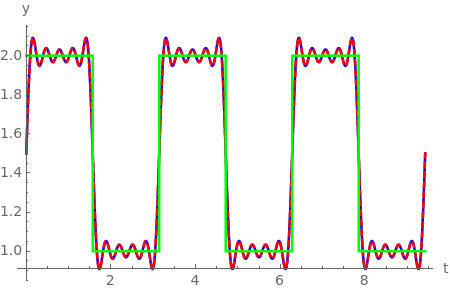
\includegraphics[width=0.45\textwidth]{pic/n10.png}
    }


    \vskip 0.5cm
    \subfloat[n = 15]{%
        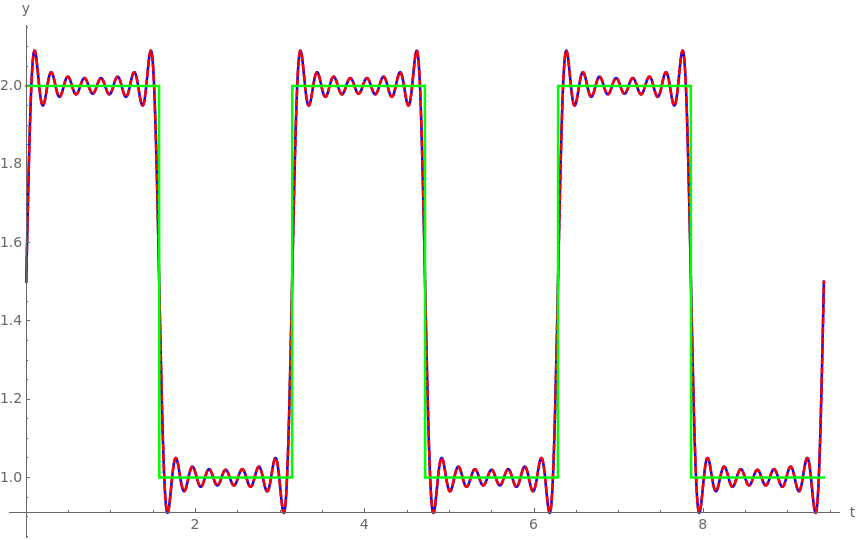
\includegraphics[width=0.7\textwidth]{pic/n15.png}
    }

    \caption{Сетка графиков}
    \label{fig:grid_plots}
\end{figure}



При небольших $n$ разложение Фурье лишь приблизительно передаёт форму квадратной волны, но с увеличением $n$ оно становится всё точнее, особенно в середине каждого интервала. Однако в точках разрыва остаются характерные колебания — эффект Гиббса: даже при бесконечном числе гармоник рядом Фурье невозможно полностью устранить скачки.

При этом тригонометрическое разложение $(A + B)$ и представление через комплексные коэффициенты $c_n$ дают один и тот же результат, что показывает эквивалентность двух подходов. 

\subsubsection{Равенство Парсерваля}

Равенство Парсеваля:
\[
\frac{1}{\pi} \int_0^{\pi} |f(t)|^2 dt = \sum_{n=-\infty}^{\infty} |c_n|^2
\]

Вычислим левую часть:
\[
\frac{1}{\pi} \left( \int_0^{\pi/2} 4 \,dt + \int_{\pi/2}^{\pi} 1 \,dt \right)
= \frac{1}{\pi} \cdot \left( 2\pi + \frac{\pi}{2} \right) = \frac{5}{2}
\]

Для правой части вычислим модули нескольких коэффициентов:
\[
|c_0| = \frac{3}{2},\quad |c_{\pm1}| = \frac{2}{\pi} \approx 0.6366,\quad |c_{\pm2}| = 0
\]
\[
|c_{\pm3}| \approx \frac{2}{3\pi} \approx 0.2122,\quad |c_{\pm4}| \approx 0,\quad |c_{\pm5}| \approx \frac{2}{5\pi} \approx 0.1273
\]

Теперь сложим квадраты модулей:
\[
|c_0|^2 + 2(|c_1|^2 + |c_3|^2 + |c_5|^2) \approx 
\frac{9}{4} + 2\left(0.4053 + 0.0450 + 0.0162\right) = 2.25 + 0.9329 \approx 2.48
\]

Сумма стремится к \(\frac{5}{2}\), коэффициенты убывают, значит равенство Парсеваля выполняется.


\subsection{Четная функция}

Рассмотрим разложение в тригонометрический ряд Фурье для функции 
Я буду рассматривать эту четную периодическую функцию
\[
f_2(t) = |\cos(t)|
\]

Вот так выглядит график моей функции

\begin{figure}[H]
    \centering
    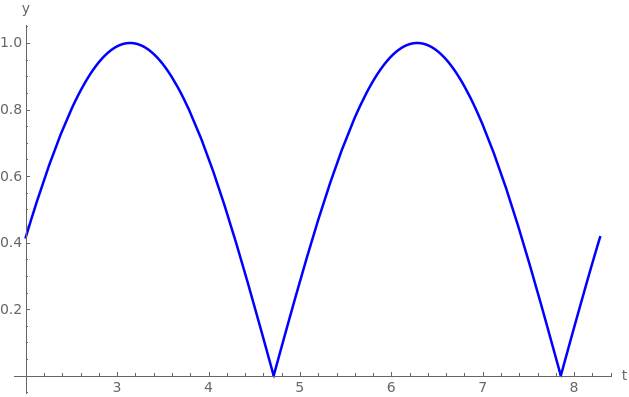
\includegraphics[width=0.7\textwidth]{pic/absCos.png}
    \caption{График $f_2(t) = |\cos(t)| $}
    \label{fig:example_image}
\end{figure}

Коэффициенты Фурье можно посчитать по формулам:

\[
a_n = \frac{2}{\pi} \int_{0}^{\pi} |\cos(x)| \cos(n x) \,dx
\]

\[
c_n = \frac{1}{\pi} \int_{0}^{\pi} |\cos(x)| e^{-i n x} \,dx
\]

\subsubsection{Программа}
Теперь напишу еще один код для счета коэффициентов Фурье
\begin{lstlisting}[language=Mathematica, caption={Код для других периодических функций}]
f2[t_] := Abs[Cos[t]];

n = 2;
h = 2;
T = 2 Pi;

p = FourierTrigSeries[f2[t], t, n];

A[i_] := (2/T) Integrate[f2[t] Cos[(2 Pi i t)/T], {t, h, h + T}];
B[i_] := (2/T) Integrate[f2[t] Sin[(2 Pi i t)/T], {t, h, h + T}];

Cc[i_] := (1/T) Integrate[f2[t] Exp[-I (2 Pi i t)/T], {t, h, h + T}];

rad = A[0]/2;
For[i = 1, i <= n, i++, 
 Print["A[", i, "] = ", A[i], "  B[", i, "] = ", B[i]];
 rad = rad + A[i] Cos[(2 Pi i t)/T] + B[i] Sin[(2 Pi i t)/T];]

For[i = -n, i <= n, i++, 
 Print["Cc[", i, "] = ", Re[Cc[i]], " + I * ", Im[Cc[i]]];]

radComplex = 
  Sum[Re[Cc[i]] Cos[(2 Pi i t)/T] - 
    Im[Cc[i]] Sin[(2 Pi i t)/T], {i, -n, n}];


Plot[{rad, radComplex, f2[t]}, {t, h, h + T}, 
 PlotStyle -> {{Thick, Blue}, {Thick, Dashed, Red}, {Thick, Green}}, 
 PlotLabel -> "Сравнение рядов Фурье", AxesLabel -> {"t", "y"}, 
 PlotRange -> All, 
 PlotLegends -> {"Реальный ряд Фурье", "Комплексный ряд Фурье", 
   "Исходная функция"}]
p
N[rad]
N[radComplex]
\end{lstlisting}

Теперь посмотрим на вывод. Сначала оценим ряды Фурье. Вот, что вывел код для $n = 2$ 
\begin{figure}[H]
    \centering
    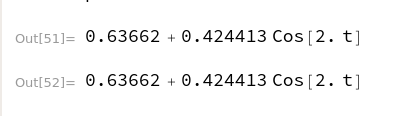
\includegraphics[width=0.4\textwidth]{pic/out2.png}
    \caption{Вывод. Ряды фурье для $f_2(t) = |\cos(t)| $}
    \label{fig:fourier_series}
\end{figure}


Можем заметить, что они одинаковые, значит задача успешно выполнена. Также уточню, что можно выводить красивые формулы без дробных чисел, с использованием числа $\pi$ , но мне больше нравится такой вывод. \\

На 7 строчке в моем коде можно заметить строчку $p = FourierTrigSeries[f2[t], t, n];$. Функция $FourierTrigSeries$ сама считает коэффициенты Фурье используя возможности языка программирования, использовалась мной для собственной проверки, проверка прошла успешно. \\


\subsubsection{Графики для больших n}
Теперь рассмотрим как поведут себя ряды Фурье при большом количестве гармоник. Возьму такие же $n$, которые я брала для квадратной волны. \\

Тут также можно заметить, что тригонометрический и комплексные ряды Фурье совпадают, также хорошо видно, как улучшается аппроксимация при увеличени $n$.

\begin{figure}[H]
    \centering

    \subfloat[n = 4]{%
        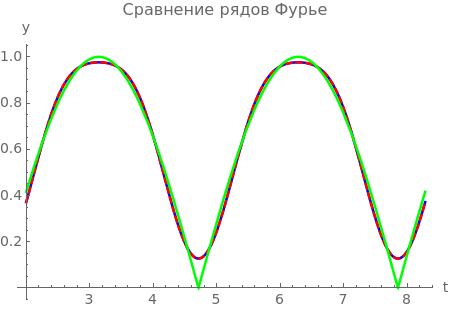
\includegraphics[width=0.45\textwidth]{pic/absCosn4.png}
    }
    \hfill
    \subfloat[n = 5]{%
        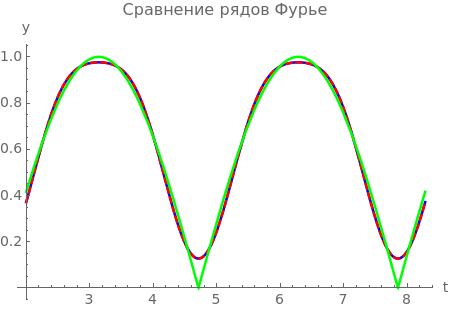
\includegraphics[width=0.45\textwidth]{pic/absCosn5.png}
    }
    
    
    \vskip 0.5cm  
    \subfloat[n = 7]{%
        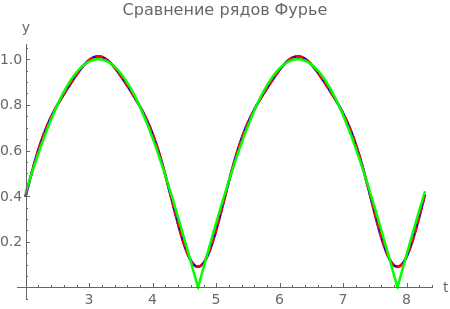
\includegraphics[width=0.45\textwidth]{pic/absCosn7.png}
    }
    \hfill
    \subfloat[n = 10]{%
        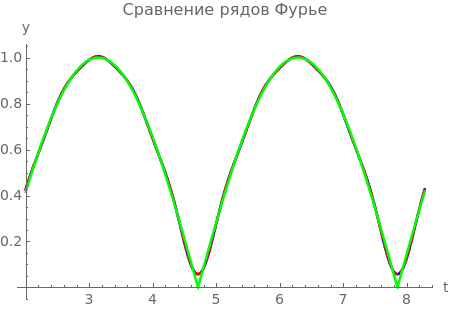
\includegraphics[width=0.45\textwidth]{pic/absCosn10.png}
    }


    \vskip 0.5cm
    \subfloat[n = 15]{%
        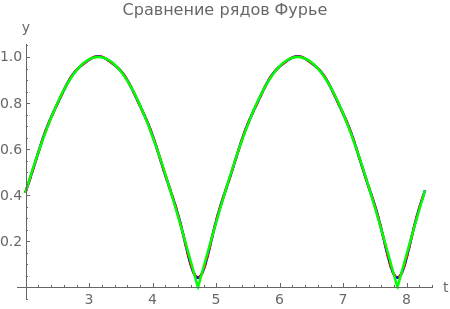
\includegraphics[width=0.7\textwidth]{pic/absCosn15.png}
    }

    \caption{Сетка графиков}
    \label{fig:grid_plots}
\end{figure}



\subsubsection{Равенство Парсерваля}

Вычислим интеграл:
\[
\frac{1}{2\pi} \int_{-\pi}^{\pi} |\cos(t)|^2 dt = \frac{1}{2\pi} \int_{-\pi}^{\pi} \cos^2(t)\,dt = \frac{1}{2}
\]

Теперь рассмотрим сумму квадратов модулей коэффициентов Фурье:
\[
|c_0|^2 = \left( \frac{2}{\pi} \right)^2 \approx 0.405,\quad |c_2|^2 \approx 0.25,\quad |c_4|^2 \approx 0.03,\quad |c_6|^2 \approx 0.005,\quad \ldots
\]

Сумма:
\[
\sum |c_n|^2 \approx 0.405 + 0.25 + 0.03 + 0.005 + \dots \approx 0.5
\]

Равенство Парсеваля выполняется.


\subsection{Нечетная функция}

В качестве нечетной функции я выбрала 

\[
f_2(t) = \sin(3t) + t
\]

Коэффициенты \( a_n \) и \( b_n \) вычисляются по формулам:
\[
a_n = 0 \quad \text{для всех } n \geq 1.
\]

\[
b_n = \frac{1}{\pi} \int_{-\pi}^{\pi} \left( \sin(3t) + t \right) \sin(nt) \, dt.
\]


Коэффициенты \( c_n \) вычисляются по формуле:
\[
c_n = \frac{1}{2\pi} \int_{-\pi}^{\pi} \left( \sin(3t) + t \right) e^{-i n t} \, dt \quad (n \in \mathbb{Z}).
\]

И вот так я изобразила функцию
\begin{figure}[H]
    \centering
    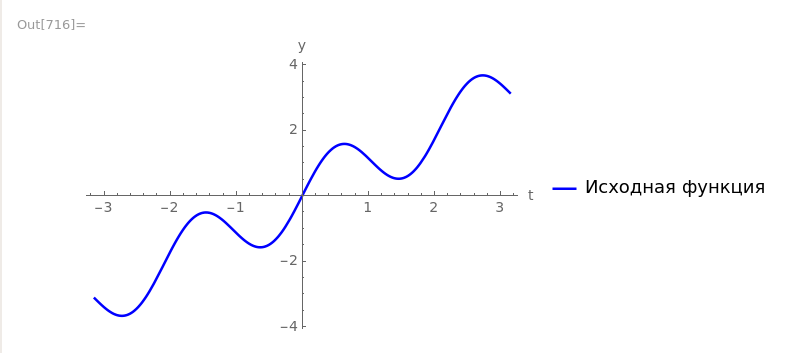
\includegraphics[width=0.7\textwidth]{pic/sin.png}
    \caption{График функции $f(t) = \sin(3t) + t$}
    \label{fig:fourier_series}
\end{figure}

\subsubsection{Код для нечетной функции}

Стоит обратить внимание, что в программе прописаны другие параметры $h$ и $T$.

\begin{lstlisting}[language=Mathematica, caption={Код для нечетной функции}]

f[t_] := Sin[3 t] + t

n = 5;
h = -\[Pi];
T = 2 \[Pi];

A[i_] := (2/T) Integrate[f[t] Cos[(2 Pi i t)/T], {t, h, h + T}];
B[i_] := (2/T) Integrate[f[t] Sin[(2 Pi i t)/T], {t, h, h + T}];

Cc[i_] := (1/T) Integrate[f[t] Exp[-I (2 Pi i t)/T], {t, h, h + T}];

rad = A[0]/2;
For[i = 1, i <= n, i++, 
 Print["A[", i, "] = ", A[i], "  B[", i, "] = ", B[i]];
 rad = rad + A[i] Cos[(2 Pi i t)/T] + B[i] Sin[(2 Pi i t)/T];]

For[i = -n, i <= n, i++, 
 Print["Cc[", i, "] = ", Re[Cc[i]], " + I * ", Im[Cc[i]]];]

radComplex = 
  Sum[Re[Cc[i]] Cos[(2 Pi i t)/T] - 
    Im[Cc[i]] Sin[(2 Pi i t)/T], {i, -n, n}];

Plot[{rad, radComplex, f[t]}, {t, h, h + T}, 
 PlotStyle -> {{Thick, Blue}, {Thick, Dashed, Red}, {Thick, Green}}, 
 AxesLabel -> {"t", "y"}, PlotRange -> All, 
 PlotLegends -> {"Реальный ряд Фурье", "Комплексный ряд Фурье", 
   "Исходная функция"}]

N[rad]
N[radComplex]

Plot[f[t], {t, h, h + T}, PlotStyle -> {Thick, Blue}, 
 AxesLabel -> {"t", "y"}, PlotRange -> All, 
 PlotLegends -> {"Исходная функция"}]
\end{lstlisting}

Программа написана, теперь можно посмотреть на ряды Фурье при $n = 2$.
Вот что вывелось мне при просмотре соответствующих переменных

\begin{figure}[H]
    \centering
    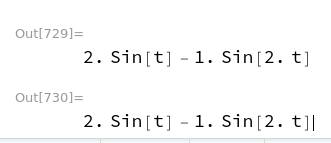
\includegraphics[width=0.4\textwidth]{pic/out3.png}
    \caption{Вывод. Ряды Фурье для $f(t) = \sin(3t) + t$}
    \label{fig:fourier_series}
\end{figure}

Отлично, они полностью совпадают и я в очередной раз убеждаюсь в верности задания(конечно, в случае, если не допущены идентичные ошики при расчете вещественных и комплексных коэффициентов Фурье). \\
Теперь посмотрим на график и сравним функцию с апроксимированной при $n = 2$

\begin{figure}[H]
    \centering
    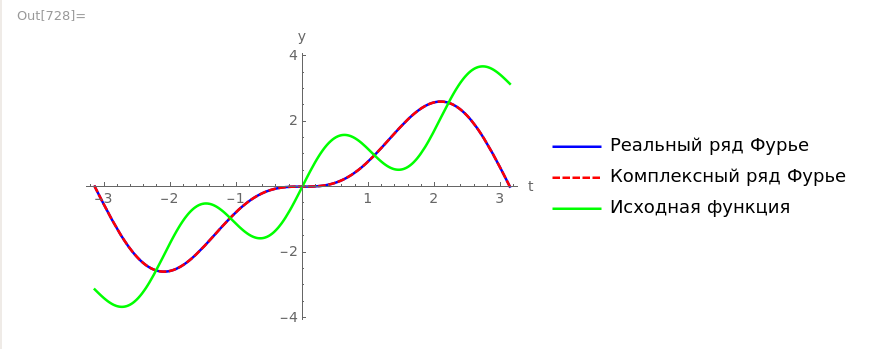
\includegraphics[width=0.8\textwidth]{pic/sinn2.png}
    \caption{Вывод. Функция и ряды Фурье для $f(t) = \sin(3t) + t$}
    \label{fig:fourier_series}
\end{figure}

Убеждаюсь, что функции сумм Фурье совпадают, а также не очень хорошо апроксимируют функцию. Теперь рассмотрю графики для большего числа гармоник.

\subsubsection{Графики для нечетной функции}

\begin{figure}[H]
    \centering

    \subfloat[n = 4]{%
        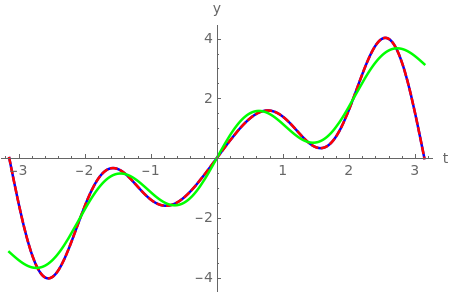
\includegraphics[width=0.45\textwidth]{pic/sinn4.png}
    }
    \hfill
    \subfloat[n = 5]{%
        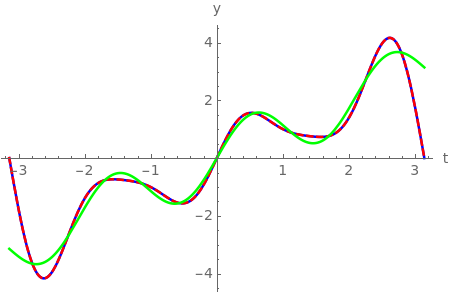
\includegraphics[width=0.45\textwidth]{pic/sinn5.png}
    }
    
    
    \vskip 0.5cm  
    \subfloat[n = 7]{%
        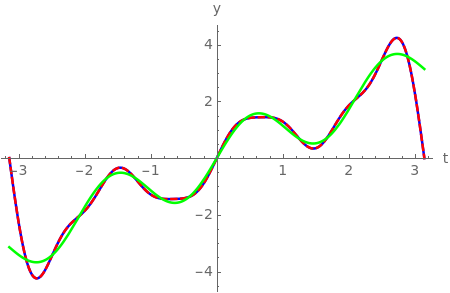
\includegraphics[width=0.45\textwidth]{pic/sinn7.png}
    }
    \hfill
    \subfloat[n = 10]{%
        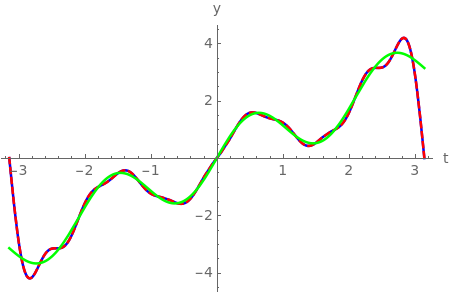
\includegraphics[width=0.45\textwidth]{pic/sinn10.png}
    }


    \vskip 0.5cm
    \subfloat[n = 15]{%
        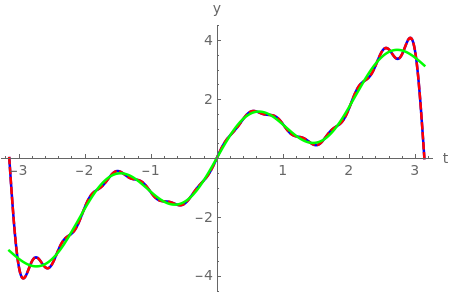
\includegraphics[width=0.7\textwidth]{pic/sinn15.png}
    }

    \caption{Сетка графиков}
    \label{fig:grid_plots}
\end{figure}

\subsubsection{Равенство Парсерваля}
Посчитаем интеграл:
\[
\frac{1}{2\pi} \int_{-\pi}^{\pi} (\sin(3t) + t)^2 dt
= \frac{1}{2} + \frac{\pi^2}{3}
\]

Теперь найдём сумму квадратов модулей коэффициентов Фурье:
\[
|c_3|^2 = \frac{1}{4}, \quad
\sum_{n \ne 0,\; n \ne \pm3} \left| \frac{i(-1)^n}{n} \right|^2 = \sum_{n=1}^{\infty} \frac{1}{n^2} = \frac{\pi^2}{6}
\]

\[
\sum |c_n|^2 = \frac{1}{4} + \frac{\pi^2}{6} + \frac{1}{4} = \frac{1}{2} + \frac{\pi^2}{3}
\]

Равенство Парсеваля выполняется.
\subsection{Любая периодическая функция}
По заданию нужно выбрать периодическую функцию, которая не является ни четной, ни нечетной. Я рассмотрю в этом задании функцию 
\[
f(t) = \sin(t) + \cos(2t) + 2t
\]
И зациклю ее с периодом \(2 \pi\). Аналитически это можно записать так:
\[ 
\mathrm{periodF}(t) = \sin(t) + \cos(2t) + 2\left(t - 2\pi \left\lfloor \frac{t + \pi}{2\pi} \right\rfloor \right)
\]
\subsubsection{Коэффициенты и график}


Итак, рассмотрим код для этой функции и график (поскольку лицензия на Wolfram matematica истекла, все следующие коды на Python):

\begin{lstlisting}[language=Python, caption={Код для любой периодической функции}]
def f(t):
    return np.sin(t) + np.cos(2*t) + 2*t

def periodF(t):
    tMod = (t + np.pi) % (2*np.pi) - np.pi 
    return f(tMod)
\end{lstlisting}

\begin{figure}[H]
    \centering
    
\includegraphics[width=1\textwidth]{pic/Figure_1.png}
    \caption{Моя периодическая функция \(f(t) = \sin(t) + \cos(2t) + 2t\)}
    \label{fig:fourier_series}
\end{figure}

Теперь расчитаем коэффициенты Фурье, запишу формулы, а их посчитают современные технологии:

\[
a_n = \frac{1}{\pi} \int_{-\pi}^{\pi} \left[\sin(t) + \cos(2t) + 2t\right]\cos(nt) dt
\]

\[
b_n = \frac{1}{\pi} \int_{-\pi}^{\pi} \left[\sin(t) + \cos(2t) + 2t\right]\sin(nt) dt
\]

\[
c_n = \frac{1}{2\pi} \int_{-\pi}^{\pi} \left[\sin(t) + \cos(2t) + 2t\right]e^{-int} dt
\]

Посмотрим на вывод:
\begin{lstlisting}[language=Python, caption={Вывод значений \(a_n\)}]
a0 =  0.0
a1 =  0.0
a2 =  1.0
a3 =  0.0
a4 =  -0.0
\end{lstlisting}
- Можно заметить, что почти все первые коэффициенты равны нулю, кроме \(a_2 = 1\).

\begin{lstlisting}[language=Python, caption={Вывод значений \(b_n\)}]
b0 =  0.0
b1 =  5.0
b2 =  -2.3
b3 =  1.33
b4 =  -1
\end{lstlisting}
- Тут почти все коэффициенты \(b_n\) ненулевые.

\begin{lstlisting}[language=Python, caption={Вывод значений \(c_n\)}]
c-4 = (-0-0.5j)
c-3 = 0.67j
c-2 = (0.5-1j)
c-1 = 2.5j
c0 = 0j
c1 = -2.5j
c2 = (0.5+1j)
c3 = -0.67j
c4 = (-0+0.5j)
\end{lstlisting}
- Коэффициенты симметричны относительно \(c_0\).


\subsubsection{Графики рядов Фурье}
Теперь посмотрим на графики этой функции и апроксимирующих функций для различных значений \(n\).


\begin{figure}[H]
    \centering
    
\includegraphics[width=1\textwidth]{pic/Figure_2.png}
    \caption{Аппроксимация при $n = 4$}
    \label{fig:n4}
\end{figure}

\begin{figure}[H]
    \centering
    
\includegraphics[width=1\textwidth]{pic/Figure_3.png}
    \caption{Аппроксимация при $n = 5$}
    \label{fig:n5}
\end{figure}

\begin{figure}[H]
    \centering
    
\includegraphics[width=1\textwidth]{pic/Figure_4.png}
    \caption{Аппроксимация при $n = 7$}
    \label{fig:n7}
\end{figure}

\begin{figure}[H]
    \centering
    
\includegraphics[width=1\textwidth]{pic/Figure_5.png}
    \caption{Аппроксимация при $n = 10$}
    \label{fig:n10}
\end{figure}

\begin{figure}[H]
    \centering
    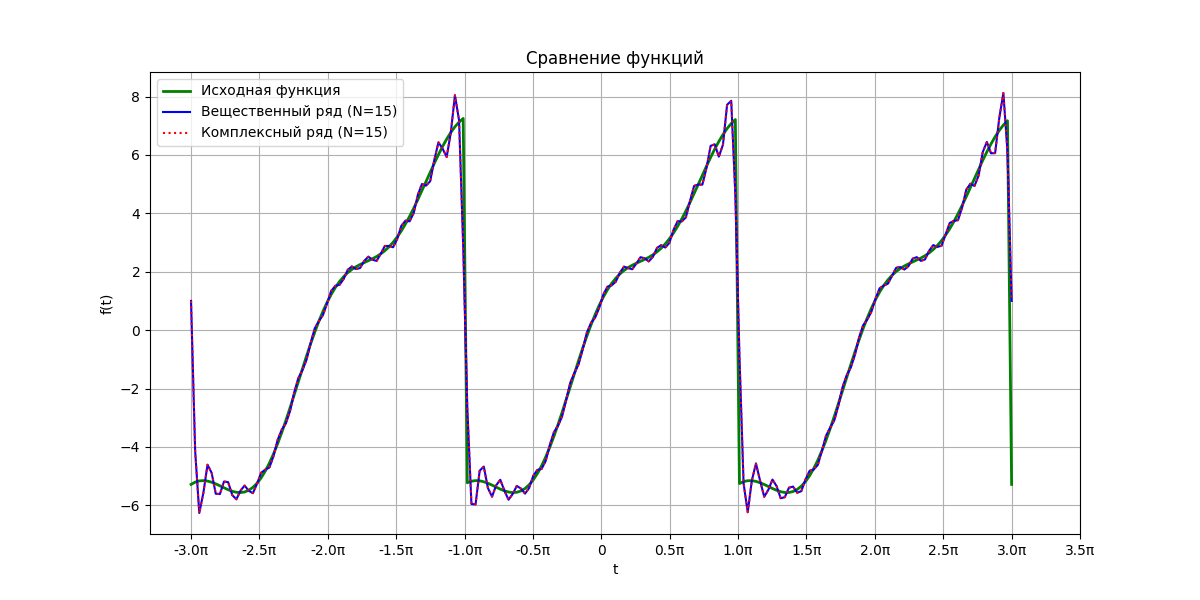
\includegraphics[width=1\textwidth]{pic/Figure_6.png}
    \caption{Аппроксимация при $n = 15$}
    \label{fig:n15}
\end{figure}

Итак, все работает корректно, с увеличением n увелисивается число гармоник  точность аппроксимации. Однако увеличивается эффект Гиббса: в концах периодов лишний "хвостик" становится все выше.
\subsubsection{Равенство Парсеваля}


\section{Task. Комплексные функции}

\subsection{Аналитические выкладки}
В этом задании нужно выбрать параметры для такой функции и подставить их туда. 
\[
\Re(f(t)) =
\begin{cases}
R, & t \in \left[-\frac{T}{8},\,\frac{T}{8}\right), \\
2R - \frac{8Rt}{T}, & t \in \left[\frac{T}{8},\,\frac{3T}{8}\right), \\
-R, & t \in \left[\frac{3T}{8},\,\frac{5T}{8}\right), \\
-6R + \frac{8Rt}{T}, & t \in \left[\frac{5T}{8},\,\frac{7T}{8}\right),
\end{cases}
\qquad
\Im(f(t)) =
\begin{cases}
\frac{8Rt}{T}, & t \in \left[-\frac{T}{8},\,\frac{T}{8}\right), \\
R, & t \in \left[\frac{T}{8},\,\frac{3T}{8}\right), \\
4R - \frac{8Rt}{T}, & t \in \left[\frac{3T}{8},\,\frac{5T}{8}\right), \\
-R, & t \in \left[\frac{5T}{8},\,\frac{7T}{8}\right),
\end{cases}
\]
В моем случае \(R = 1\) и \(T = 2\). Посмотрим на получившуюся функцию:
\[
\Re(f(t)) =
\begin{cases}
1, & t \in \left[-\frac{1}{4},\,\frac{1}{4}\right), \\
2 - 4t, & t \in \left[\frac{1}{4},\,\frac{3}{4}\right), \\
-1, & t \in \left[\frac{3}{4},\,\frac{5}{4}\right), \\
-6 + 4t, & t \in \left[\frac{5}{4},\,\frac{7}{4}\right),
\end{cases}
\qquad
\Im(f(t)) =
\begin{cases}
4t, & t \in \left[-\frac{1}{4},\,\frac{1}{4}\right), \\
1, & t \in \left[\frac{1}{4},\,\frac{3}{4}\right), \\
4 - 4t, & t \in \left[\frac{3}{4},\,\frac{5}{4}\right), \\
-1, & t \in \left[\frac{5}{4},\,\frac{7}{4}\right),
\end{cases}
\]

\begin{figure}[H]
    \centering
    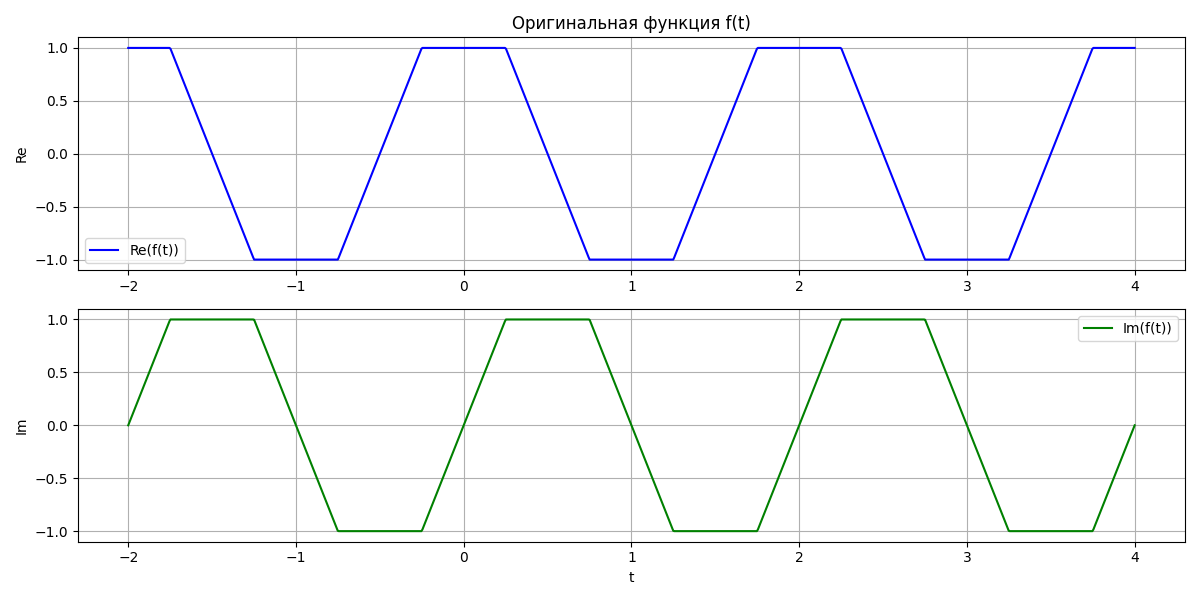
\includegraphics[width=1\textwidth]{pic2/ich.png}
    \caption{Исходная функция}
    \label{fig:n5}
\end{figure}


В общем виде выведу формулу для подсчета коэффициентов:

\[
c_n = \frac{1}{T} \int_{-T/2}^{T/2} f(t)\, e^{-i \omega_n t} \, dt, \quad \omega_n = \frac{2\pi n}{T}
\]

\[
c_n = \frac{1}{T} \left[
\int_{-\frac{T}{8}}^{\frac{T}{8}} \left(R + i \cdot \frac{8Rt}{T} \right) e^{-i \omega_n t} dt +
\int_{\frac{T}{8}}^{\frac{3T}{8}} \left(2R - \frac{8Rt}{T} + iR \right) e^{-i \omega_n t} dt +
\right.
\]
\[
\left.
\int_{\frac{3T}{8}}^{\frac{5T}{8}} \left(-R + i \left(4R - \frac{8Rt}{T} \right) \right) e^{-i \omega_n t} dt +
\int_{\frac{5T}{8}}^{\frac{7T}{8}} \left(-6R + \frac{8Rt}{T} - iR \right) e^{-i \omega_n t} dt
\right]
\]



\[
\text{Подставим } T = 2,\ R = 1,\ \omega_n = \pi n:
\]

\[
c_n = \frac{1}{2} \left[
\int_{-0.25}^{0.25} \left(1 + i \cdot 4t \right) e^{-i\pi n t} dt +
\int_{0.25}^{0.75} \left(2 - 4t + i \right) e^{-i\pi n t} dt +
\right.
\]
\[
\left.
\int_{0.75}^{1.25} \left(-1 + i(4 - 4t) \right) e^{-i\pi n t} dt +
\int_{1.25}^{1.75} \left(-6 + 4t - i \right) e^{-i\pi n t} dt
\right]
\]

% При чётных n (например, n = -2, 0, 2) — половинная симметрия приводит к занулению:
\[
c_{-2} = c_0 = c_2 = 0
\]

% Отрицательные n → коэффициенты исчезают из-за односторонней спектральной природы (анализируемая функция аналитическая):
\[
c_{-1} = 0
\]

% Единственный ненулевой коэффициент:
\[
c_1 = \frac{8\sqrt{2}}{\pi^2}
\]

\subsection{Програмный вывод коэффициентов}
Посмотрим на функцию, которая считает коэффициенты Фурье:

\begin{lstlisting}[language=Python, caption={Функция коэффициентов \(c_n\)}]
def cN(n, T=T):
    omega_n = 2 * np.pi * n / T
    integrand = lambda t: f(t, T) * np.exp(-1j * omega_n * t)
    return (1/T) * quad(integrand, -T/2, T/2, complex_func=True)[0]
\end{lstlisting}

И посмотрим, что выведет применение этой функции для N = 2:

\begin{lstlisting}[language=Python, caption={Вывод коэффициентов \(c_n\)}]
=== Коэффициенты Фурье при N = 2 ===
c_-1 = -0.000000 + 0.000000j  | |c_-1| = 0.000000
c_0 = 0.000000 + 0.000000j  | |c_0| = 0.000000
c_1 = 1.146318 + 0.000000j  | |c_1| = 1.146318
\end{lstlisting}

Итак, они сходятся с вычисленными аналитически.

\subsection{Параметрические графики}

На одном графике я построю параметрические графики частичных сумм
ряда при \( N = \{1,\ 2,\ 3,\ 10\} \)


\begin{figure}[H]
    \centering
    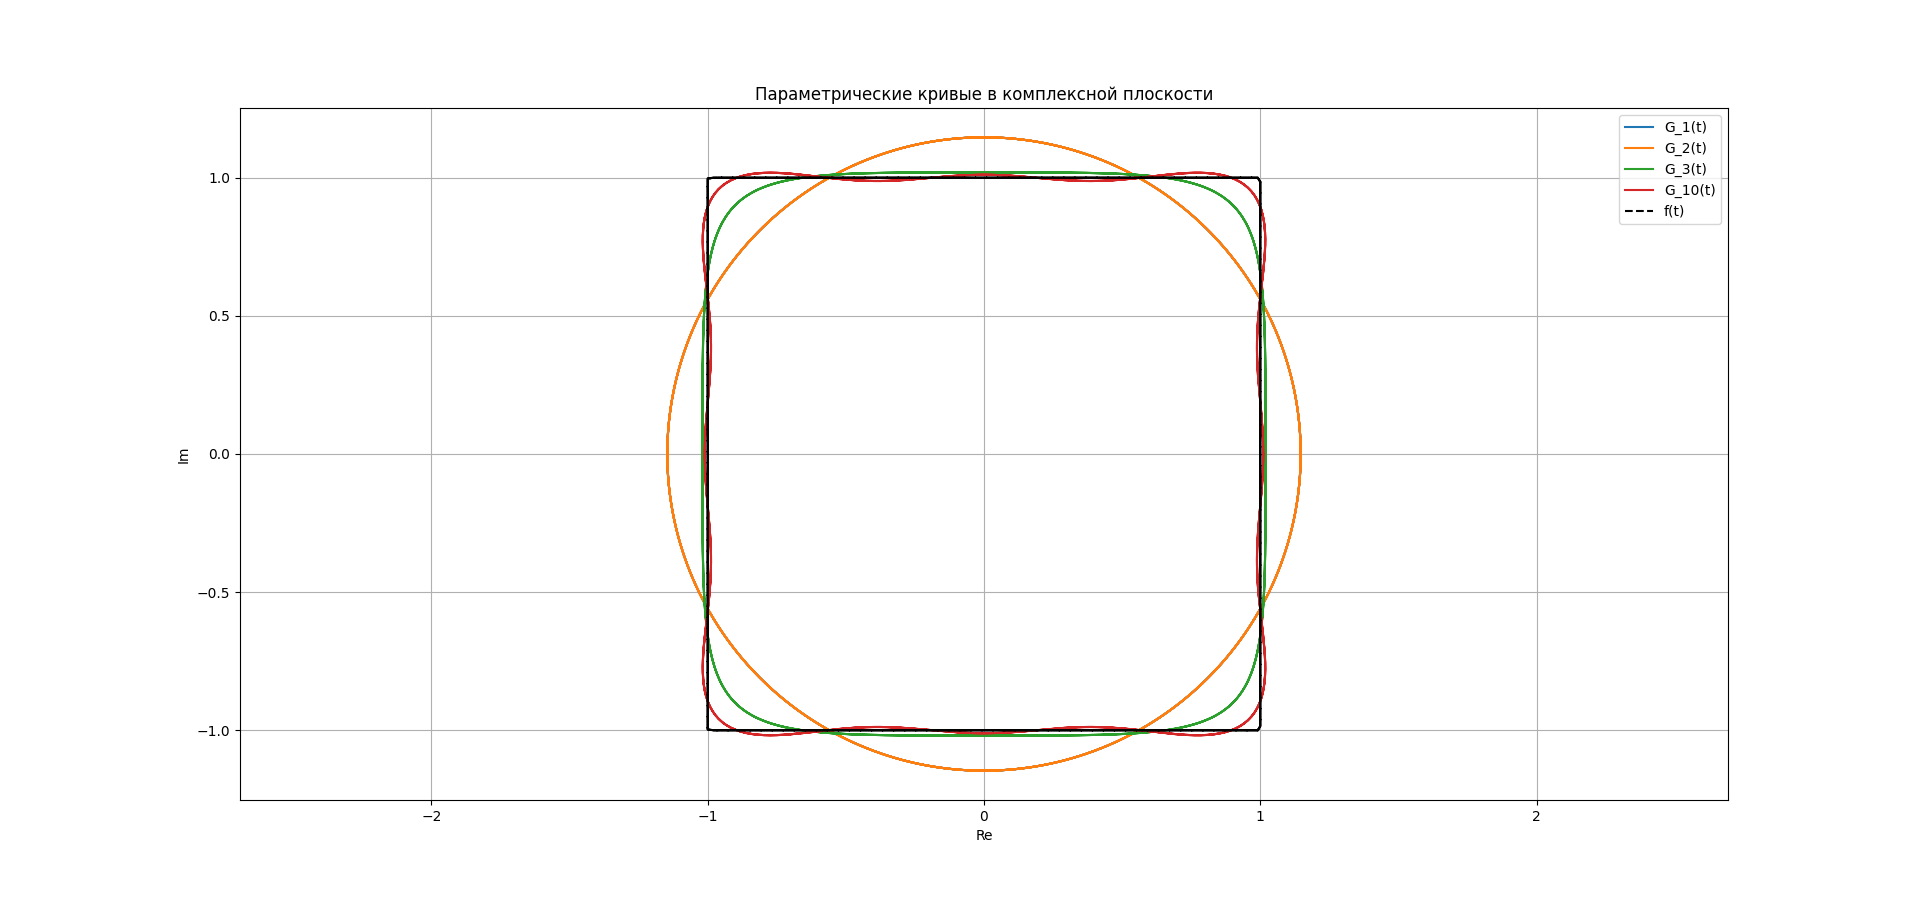
\includegraphics[width=1\textwidth]{pic2/par.png}
    \caption{Параметрические графики}
    \label{fig:n5}
\end{figure}
\[
\text{На графике изображены траектории частичных сумм } G_N(t) \text{ в комплексной плоскости.}
\]
\[
\text{Каждая кривая отображает зависимость } G_N(t) = \Re(G_N(t)) + i\,\Im(G_N(t)) \text{ при фиксированном } N.
\]
\[
\text{Черная линия соответствует исходной функции } f(t),\ \text{а остальные — приближённым рядам Фурье.}
\]

\subsection{Построение графиков}

Теперь построю графики \(\Re(G_N(t))\) и \(\Im(G_N(t))\) при \( N = \{1,\ 2,\ 3,\ 10\} \)
и сравню их с графиками \(\Re(f(t))\) и \(\Im(f(t))\).
Это позволит наглядно увидеть, как частичные суммы ряда Фурье приближают исходную функцию
при увеличении числа гармоник.


\begin{figure}[H]
    \centering
    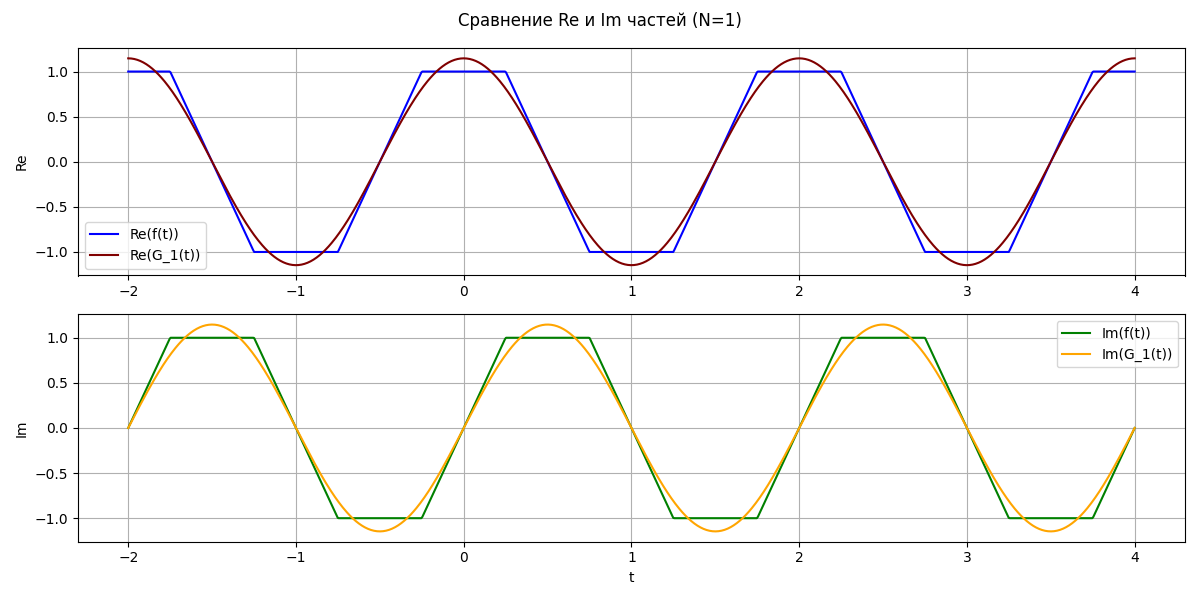
\includegraphics[width=1\textwidth]{pic2/g1.png}
    \caption{\(N = 1\)}
    \label{fig:n5}
\end{figure}


\begin{figure}[H]
    \centering
    
\includegraphics[width=1\textwidth]{pic2/g2.png}
    \caption{\(N = 2\)}
    \label{fig:n5}
\end{figure}


\begin{figure}[H]
    \centering
    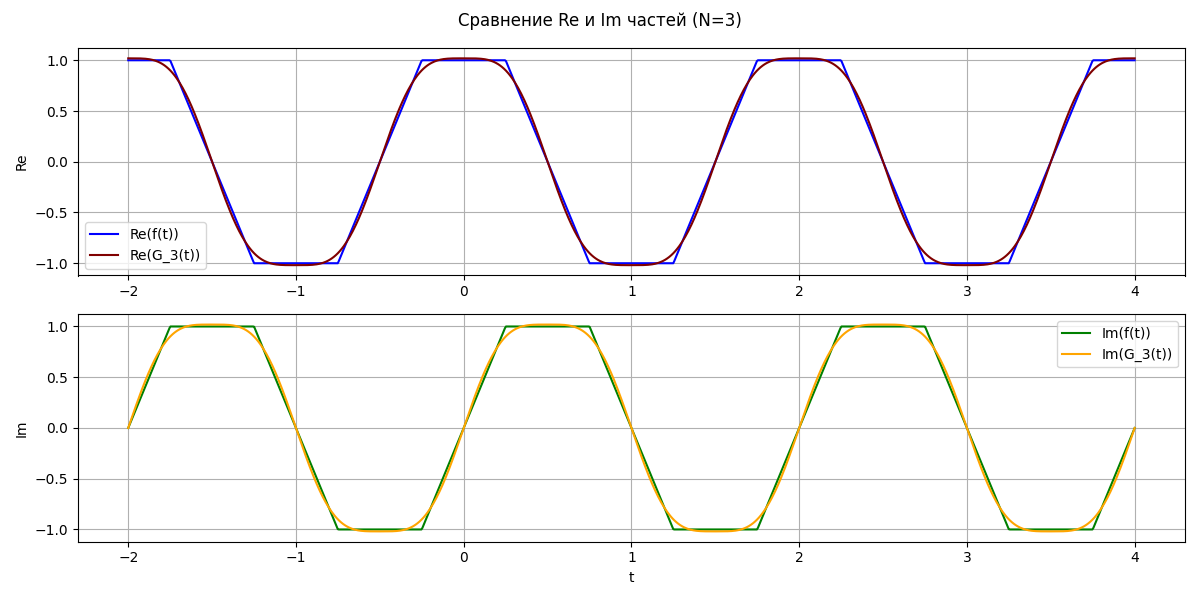
\includegraphics[width=1\textwidth]{pic2/g3.png}
    \caption{\(N = 3\)}
    \label{fig:n5}
\end{figure}


\begin{figure}[H]
    \centering
    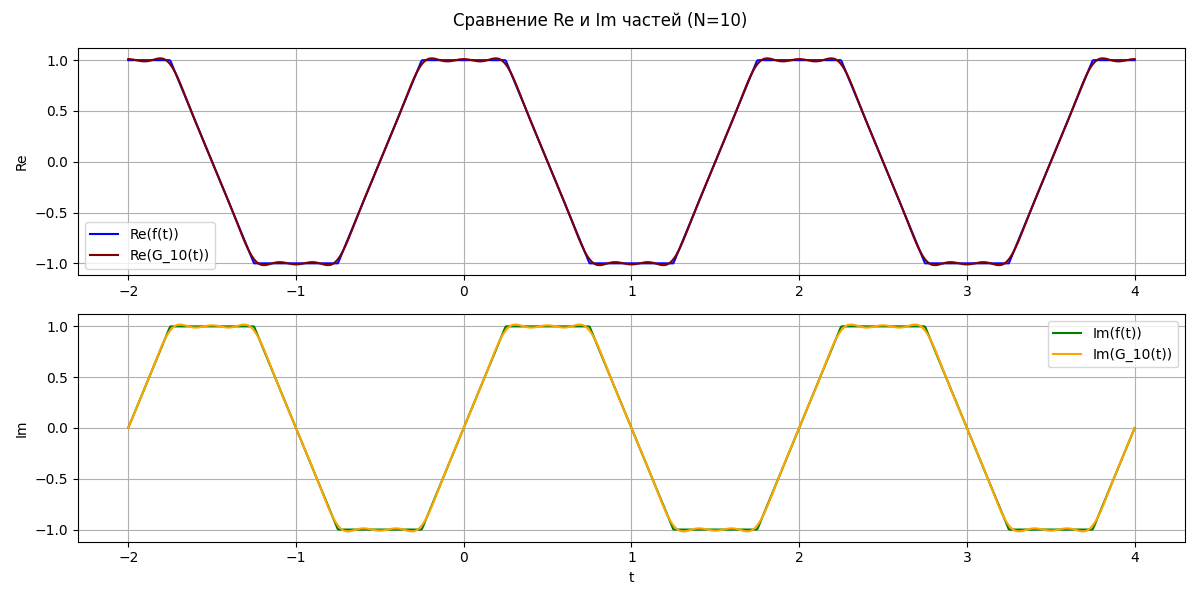
\includegraphics[width=1\textwidth]{pic2/g4.png}
    \caption{\(N = 10\)}
    \label{fig:n5}
\end{figure}

Сравнение графиков показывает, что при увеличении числа гармоник \( N \)
частичная сумма ряда Фурье \( G_N(t) \) всё точнее приближает исходную функцию \( f(t) \).
Для малых \( N \) заметны сглаженные участки и отклонения от формы \( f(t) \),
но при \( N = 10 \) графики практически совпадают, особенно вне точек разрыва.


\subsection{Равенство Парсеваля}
Программно проверю выполнение равенства Парсеваля. Напишу код:

\begin{lstlisting}[language=Python, caption={Равенство Парсеваля. Функция}]
def parseval_check(T, N):
    energy_time = (1/T) * quad(lambda t: abs(f(t, T))**2, -T/2, T/2, limit=200)[0]
    energy_freq = sum(abs(cN(n, T))**2 for n in range(-N, N+1))

    print("=== Проверка равенства Парсеваля ===")
    print(f"(1/T) ∫|f(t)|² dt ≈ {energy_time:.6f}")
    print(f"∑|cₙ|² от -{N} до {N} ≈ {energy_freq:.6f}")
    print(f"Delta: {abs(energy_time - energy_freq):.6e}\n")
\end{lstlisting}

Посмотрим на вывод:

\begin{lstlisting}[language=Python, caption={Равенство Парсеваля \(N = 10\)}]
=== Проверка равенства Парсеваля ===
(1/T) ∫|f(t)|² dt ≈ 1.333333
∑|cₙ|² от -10 до 10 ≈ 1.333119
Delta: 2.147725e-04
\end{lstlisting}

Равенство Парсеваля выполнено.


\section{Выводы}

В этой лабораторной работе я научилась строить ряды Фурье для разных функций — чётных, нечётных и произвольных. Я сравнивала полученные разложения с оригинальными функциями и видела, как приближение улучшается при увеличении числа гармоник.

Также я убедилась, что разложения с помощью тригонометрических и комплексных коэффициентов дают одинаковый результат.

Было интересно наблюдать эффект Гиббса — характерные колебания возле разрывов, которые не исчезают даже при больших \( N \).

Кроме того, я проверила равенство Парсеваля и увидела, что оно действительно выполняется.

Работа получилась насыщенной и познавательной — всё, что планировала, получилось. \href{http://github.com/decadeos/ITMO/tree/master/2_course/chMetods/lab1}{GitHub} к кодами и latex.




\end{document}
